Data mining, also referred to as knowledge discovery in databases (KDD), is the nontrivial extraction of implicit, previously unknown, and potentially useful information from data~\cite{Frawley1992}. But the measure of what is meant by ``useful" to the user is dependent on the user as well as the domain within which the data mining system is being used. Therefore, the role of domain knowledge in the discovery process is essential. Fayyad \etal~\cite{Fayyad96} contended that the use of domain knowledge is important in all stages of the data mining process including, for example, data transformation, feature reduction, algorithm selection, post-processing, model interpretation and so forth.

The first step towards using domain knowledge is to acquire the knowledge from experts and thus model and codify the knowledge in the computer. Russell and Norvig~\cite{Russell03} emphasized that a data mining system must have some method for obtaining the background knowledge and can no longer make naive speculations, and should use its background knowledge to learn more and more effectively. This process of modeling knowledge in computer systems to facilitate problem solving is studied in the field of knowledge representation/engineering. Research in this field has resulted in many sophisticated technologies such as expert systems. However, at present, knowledge representation and data mining remain largely separate disciplines. Although it is widely stated that exploring the fusion of the two fields is worthwhile in many applications where substantial human expertise exists alongside data resources, as many researchers have pointed out, work along this line is still in its infancy~\cite{Hirsh94, Weiss01, Daniels01, Kopanas02, Langseth03}.

%Previous research has made few attempts to build data mining systems that are capable of incorporating domain knowledge in a generalizable way. In some of those systems where users are able to express domain knowledge, such knowledge is often specified in a very application-specific form, scope and granularity. The ad hoc manner of representing knowledge hinders the interoperability and reuse of codified knowledge~\cite{Pohle03}. Moreover, we have also noticed that in many data mining systems, domain knowledge is embedded into the implementations in the form of implicit assumptions and heuristics, which makes abstraction and refactoring particularly hard. Sometimes even data mining practitioners themselves are not aware of employing domain knowledge in such a manner.

This problem motivates us to develop a framework for explicit incorporation of domain knowledge in a data mining system so that insights can be drawn from both knowledge and data in a systematic and holistic way. We call such technology ``semantic data mining." This dissertation contributes a first step towards realizing this goal by providing a graph-based formalism and analysis methods thereof, to systematically incorporate a specific kind of ontological domain knowledge that can be directly encoded in the W3C's Resource Description Framework (RDF) triple syntax. We showcase the utility of such method by providing theoretical, methodological and empirical insights into solving some certain non-trivial data mining tasks, such as the semantic association mining as detailed later in the chapter.


Recent research in knowledge representation, particularly in the area of W3C's Semantic Web~\cite{Berners-Lee01} that seeks to embed semantic content in web pages, has led to mature standards such as the Web Ontology Language (OWL~\cite{OWL}) for authoring ontologies. An ontology is an explicit specification of a conceptualization~\cite{Gruber93}. Today, Semantic Web ontologies have become a key technology for intelligent knowledge processing, providing a framework for sharing conceptual models about a domain~\cite{Maedche03Onto}. Ontologies explicate domain knowledge hence providing a way to separate knowledge from implementations~\cite{Noy01ontologydevelopment}. Much effort has been devoted to developing tools for coding and managing OWL ontologies~\cite{Duineveld00, Knublauch04}. Ontologies are used in various contexts, particularly those dealing with information that encompasses a limited and defined domain, and where sharing data is a common necessity, such as scientific research. Prominent examples of such efforts include the Gene Ontology (GO~\cite{GO}), Unified Medical Language System (UMLS~\cite{UMLS}), and more than 300 ontologies in the NCBO (National Center for Biomedical Ontology) such as the Neural ElectroMagnetic Ontologies (NEMO~\cite{FrishkoffEtal07, FrishkoffEtal09}).


The OWL is built on the W3C's Resource Description Framework (RDF) that provides a simple model to describe information resources as a graph. The core of the framework is the RDF statements consisting of triples including a subject (the resource being described), a predicate (the property) and an object (the property value). This simple model of assertions leads to a network of information resources, interrelated by properties which establish relations, or links, between resources and property values. The term RDF Graph is defined as a set of RDF triples (which can be illustrated by a node-arc-node link). Therefore, any collection of RDF data is an RDF Graph~\cite{GraphModelRDF}.

At the same time, there has been a surge of interest in tackling the problem of mining semantically rich datasets, where objects are linked in a number of ways. In fact, many datasets of interest today are best described as a linked collection, or a graph, of interrelated objects~\cite{LinkMiningGetoor}. These graphs may represent homogeneous networks, in which there is a single-object type and link type (such as web pages connected by hyperlinks), or richer, heterogeneous networks, in which there may be multiple object and link types (such as DBpedia, a data source containing structured information from Wikipedia). Many traditional information resources and formats can be viewed as graphs or linked collections as well. Such links and their characteristics are explored, often implicitly, by well-established data analysis and mining techniques, whose formalism of the problem are however typically not based on graphs. For example, consider a simple transaction table and the problem of frequent itemset generation. An itemset is deemed frequent if its \emph{support}, i.e., the percentage of transactions which contain that itemset, is above a threshold. If we characterize the ``co-occurrence" relationship (items appearing together in a tuple) as a link between items, then the transaction table can be viewed as a graph consisting of a set of items connected by such links. Furthermore, in this sense, the problem of frequent pattern mining can be reformulated as to identify sets of nodes in the graph that are heavily connected by the co-occurrence links.

We believe the interface between domain knowledge and data mining can be achieved, to some extent, by using graph representations in which distinct sorts of knowledge that have been traditionally differently represented can be structured in a unified manner. For example, previously, one important aspect of the distinction between domain knowledge and data is the different representations for \emph{ontological} and \emph{factual} knowledge. Ontological knowledge is related to general categories, also called concepts or classes (such as those defined in OWL ontologies). Factual knowledge makes assertions about a specific situation (\eg, this specific entity belongs to a certain category, and has a certain relationship with another entity, such as those defined in knowledge bases or relational databases). However, this distinction can be obscured by the simple semantics of the RDF model given the fact that RDF allows a combined specification of both schema and data structured under this schema. Since RDF's abstract triple syntax has a graph nature, and graphs are one of the most fundamental objects studied in mathematics that have a strong relation with logical languages and data structures, it is promising to develop graph-based approaches that provide a common ground to interface with both domain knowledge and data mining. Therefore, in this dissertation, we explore a particular graph-based method for modeling both knowledge and data, and for analyzing the combined information source from which insight can be derived systematically. We expect this novel paradigm to contribute to the development of new principles towards semantic data mining.

%\here Another kind of knowledge is implicit knowledge described. for instance. by rules of form ``if this then that" (e.g.. ``if there is a relation r from x to v, then the same relation r also holds from y to x"). Different kinds of rules can be considered. Some rules can be included in an ontology (e.g.. the transitivity of a binary relation), other rules, for instance representing possible transformations, are not ontological knowledge. Constraints, i.e., conditions that are to he fulfilled by some pieces of knowledge in order to be correctly processed by a reasoning engine, frequently appear in modeling and should be differentiated from other kinds of knowledge.

\begin{figure}[tbh]
\begin{center}
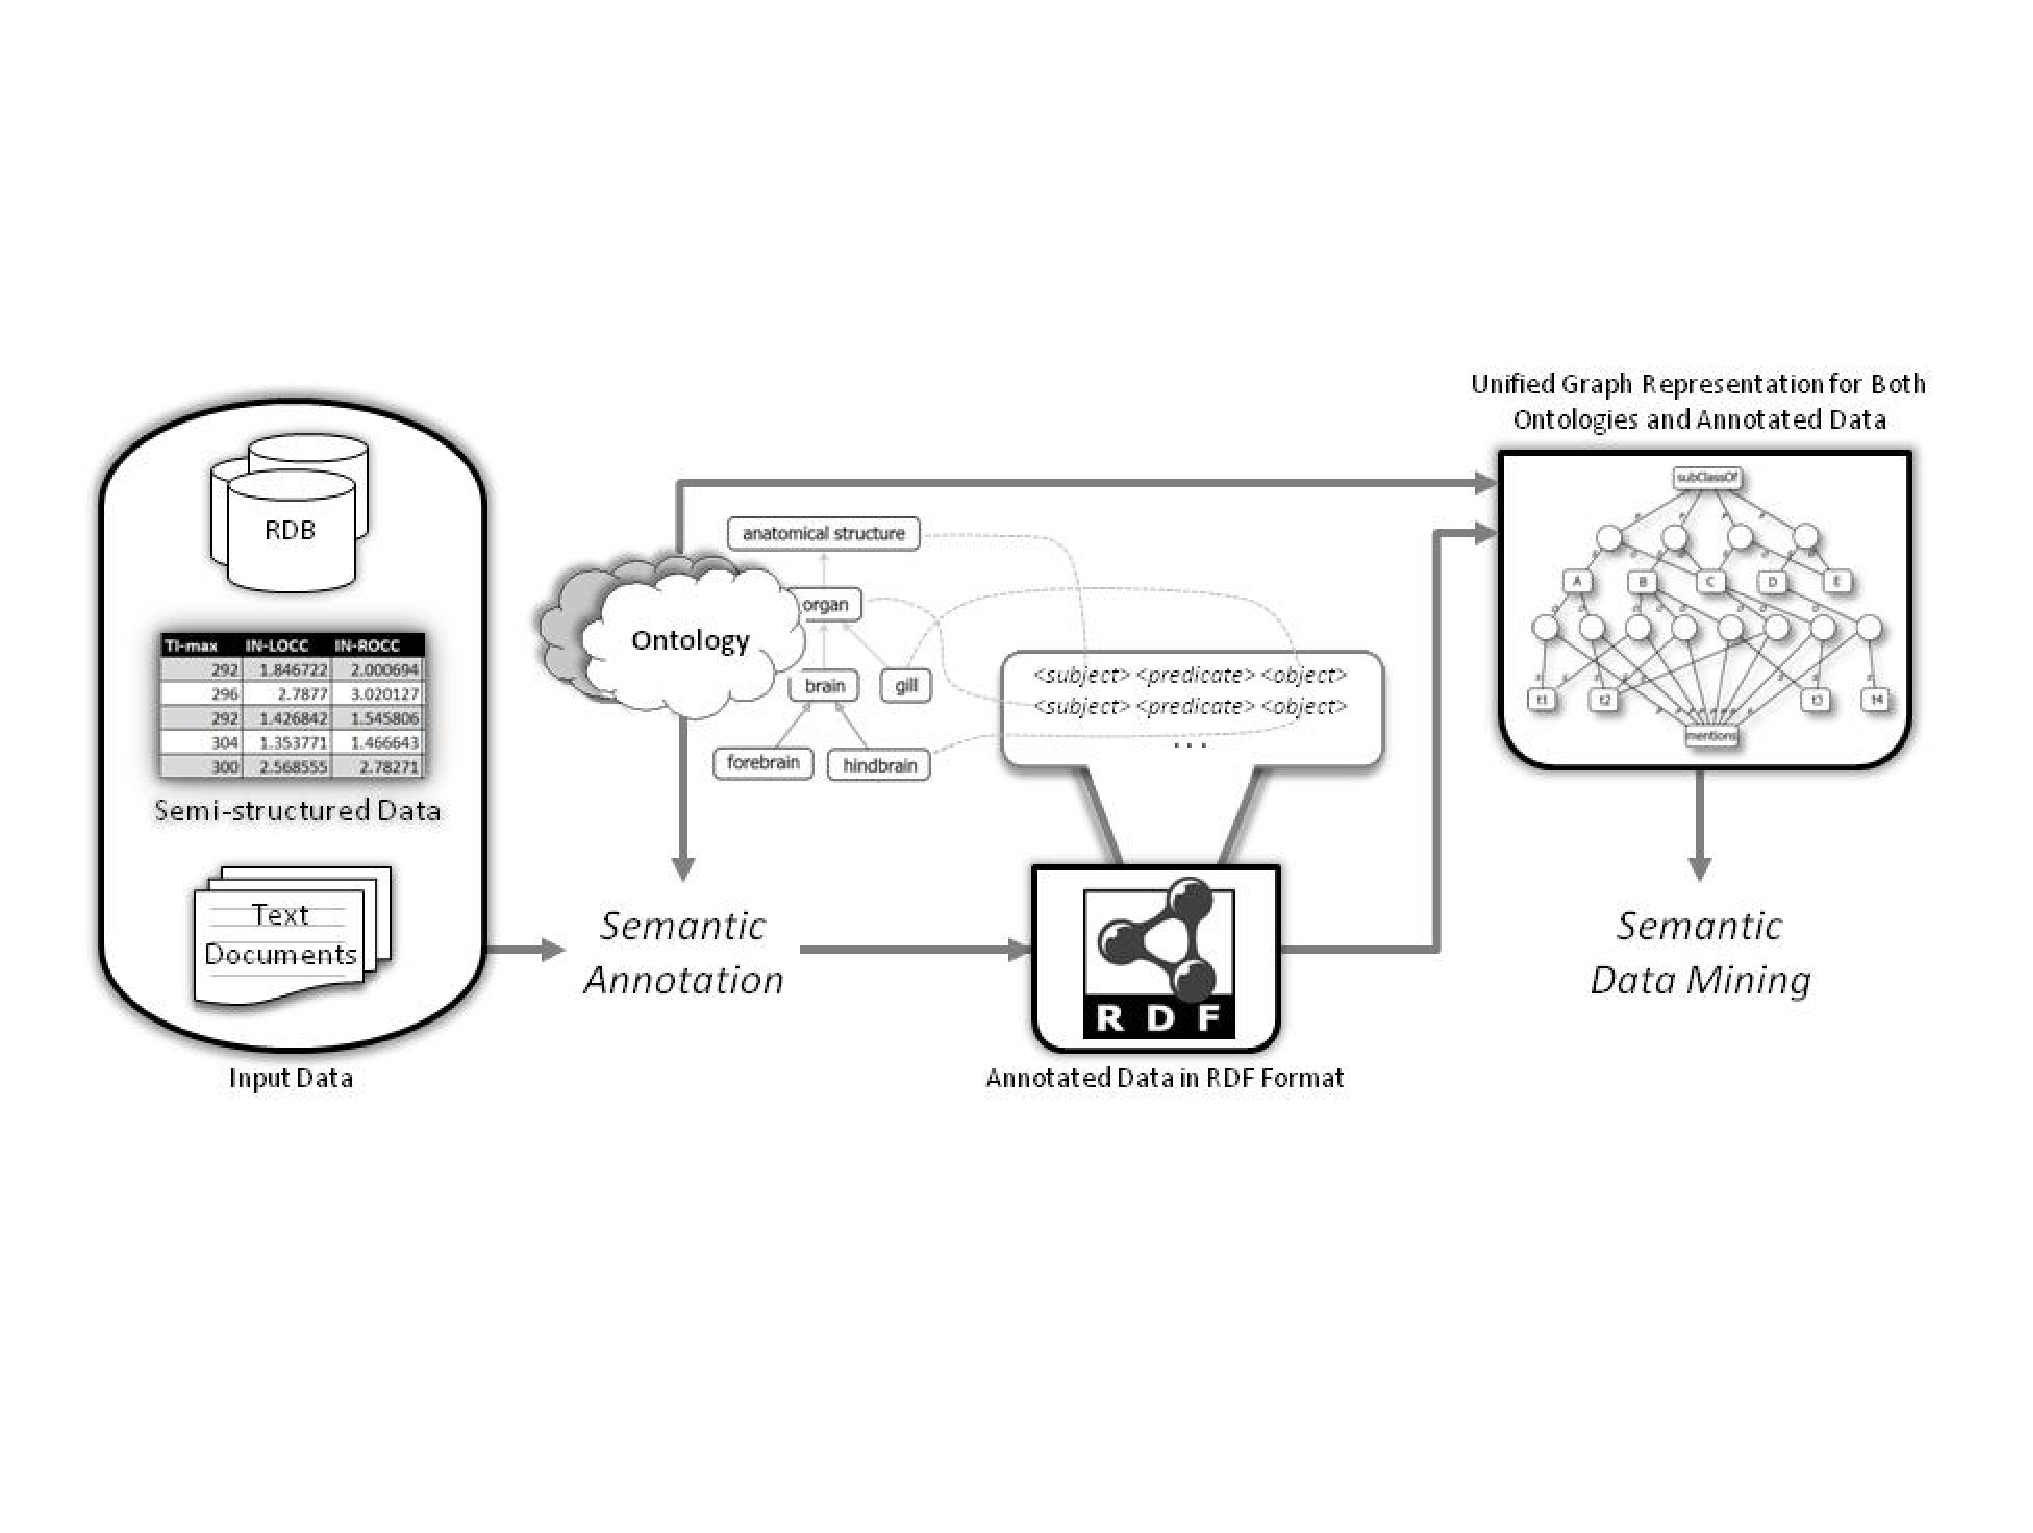
\includegraphics[width=\textwidth, trim=0 7cm 0 6cm, clip=true]{fig/thesis-semantic-annotation-workflow.eps}
\end{center}
\caption[Semantic annotation in the workflow of semantic data mining.]{\label{fig:annotation-workflow} The proposed workflow for semantic data mining.}
\end{figure}

Figure~\ref{fig:annotation-workflow} illustrates the proposed workflow for semantic data mining. Starting from a source of input data in some certain format, the first step is to identify suitable ontologies that encode concepts and relationships needed to describe the domain. Then semantic annotation is performed to link the basic element of data with formal semantic descriptions in ontologies~\cite{KiryakovEtal04}. Next, a growing number of mining tasks require an integration step to be performed in order to access and derive insights from heterogeneous information sources. Finally, the integrated data can be stored in the RDF format and be represented, together with the ontologies, by an expressive and flexible graph model for subsequent analyses.

Since graph-based semantic data mining is a new field, many interesting research directions related to it are yet to be explored. This dissertation studies three such research directions. Brief descriptions of these directions are presented below.

\begin{enumerate}
\item \textbf{A graph representation for both domain knowledge and data mining:}
    The interface between knowledge representation and data mining is achieved by employing the RDF model and by the fact that RDF allows a combined specification of both schema and data structured under this schema. RDF's ability to represent disparate, abstract concepts has led to its increasing use in knowledge representation. The RDF core vocabulary and the RDF Schema provide the most basic predefined concepts to express express schematic information. ``Richer" schema and ontology defining languages (e.g., OWL) that are built upon RDF continue to evolve.

    On the other hand, in practice, vast amounts of data often persist in relational databases (RDB). Mapping from RDB to RDF has gained increasing attention and led to the implementation of generic mapping tools as well as domain--specific applications.  The W3C launched the RDB2RDF incubator group to explore issues involved in mapping RDB to RDF~\cite{RDB2RDF}. An outstanding advantage of expressing data in RDF is the explicit modeling of relationships between entities that are either implicit or non--existent in RDB. In this way, one can achieve the incorporation of ``domain semantics," an important aspect to fully leverage the expressivity of RDF models that enables data mining systems to explore beyond pure data. Furthermore, the role of RDF as an integration platform for data from multiple sources is another main motivation for mapping RDB to RDF.

    RDF's abstract triple syntax has a graph nature. Graphs are mathematical objects that enjoy wide-spread usage for many tasks, which include the visualization and analysis of data for humans, mathematical reasoning, and the implementation as a data structure for developing data mining algorithms. Besides the common graph-theoretic model of RDF as labeled, directed multi-graphs, Hayes has established that RDF can be also represented as hypergraphs (bipartite graphs)~\cite{GraphModelRDF}. This result constitutes an important aspect of the theoretical basis of this dissertation and is discussed in Chapter II. Our novel contribution is a set of methods to represent data in relational structures using graphs in ways that are consistent with the RDF hypergraph/bipartite representation. The unified graph representation for both the data and domain knowledge encoded in ontologies is the basis for developing meaningful semantic data mining algorithms.
    
\item \textbf{An advanced method to enable data integration and meta-analysis at the same time:}
    The presence of heterogeneity among schemas and ontologies supporting vast amounts of information demands advanced solution for semantic integration of disparate data sources to facilitate interoperability and reuse of the information. Another challenging task given multiple data sources is to carry out meaningful meta-analysis that combines results of several studies on different datasets to address a set of related research hypotheses.

    We identify two prominent problems in enabling data integration and meta-analysis, namely, attribute matching and cluster matching. It can be shown that these two problems are interlocked with each other and cannot be solved separately. Therefore we develop a solution that casts them to combinatorial optimization problems with distinct yet interrelated objective functions. The core idea is a novel approach using multi-objective heuristics to discover attribute matching and cluster matching simultaneously. Details of the methods are presented in Chapter IV.

\item \textbf{A graph theoretic analysis approach for mining the combined information source of both data and knowledge:}

    %Using graph-based formalisms can bring new perspectives to traditional data mining tasks. For example, as mentioned before, the problem of frequent pattern mining can be reformulated as to identify sets of nodes that are heavily connected by the co-occurrence link. It is evident that the traditional measure of support is essentially restrained to only take into account direct links between items while ignoring the indirect ones. A prominent example of such indirect association was given by Swanson's land mark paper published in 1987~\cite{swanson87} before the age of Web-scale computation:
    %Let A stand for dietary fish oil; let B stand for a set of certain changes in the blood and circulatory system; and let C stand for the amelioration of Raynaud's syndrome, a peripheral circulatory disorder. Swanson was the first to hypothesize that dietary fish oil might benefit people afflicted with Raynaud's syndrome (A is associated with C) given that it had been already widely known that dietary fish oil causes certain blood changes (A is associated with B) and that these same blood changes may ameliorate Raynaud's syndrome (B is associated with C). The latter two associations were supported by substantial bodies of evidence but were mutually isolated and apparently had never been brought together in print. Without discovering that indirect association (A and C) a potentially useful hypothesis that is worth testing would have been missed. A graph-based analysis approach is particularly suitable to effectively discover this kind of pattern.

    %In the context of a graph model for RDF, it is useful to introduce some kind of distance metric between information resources to approach the intuitive notion of relatedness between resources. With a reasonable graph model as well as a meaningful distance metric defined, many mining problems hard to be solved by conventional methods can be tackled in a new angle with the ability to tap on domain knowledge expressed in the graph model.

    The particular mining problem we aim to solve in this dissertation is motivated by a simple scenario illustrated by Swanson~\cite{swanson87} years ago while studying Raynauld's syndrome.  He noticed that the literature discussed Raynauld's syndrome ($Z$), a peripheral circulatory disease, together with certain changes of blood in human body ($Y$); and, separately, the consumption of dietary fish oil ($X$) was also linked in the literature to similar blood changes.  But fish oil and Raynauld's syndrome were never linked directly in any previous studies.  Swanson reasoned (correctly) that fish oil could potentially be used to treat Raynauld's syndrome, i.e., $X\rightsquigarrow Y \rightsquigarrow Z$. We call such indirectly associated items, $(X,Z)$, \emph{semantically associated itemsets}.

    Our approach is based on the RDF hypergraph/bipartite representation to capture both ontologies and data. We can weight each hyperedge so that certain links can carry appropriate strength. Then, drawing inspiration from a rich body of literature on graph mining and graph spectral analysis, we explore some highly efficient and scalable similarity measures over the bipartite graph to generate frequent itemsets, including associations that may not necessarily be co-frequent. Details of these approaches are presented in Chapter V and VI.
    %At the same time, we notice that these problems may be more challenging in the graph domain due to the cost of the greater expressive power associated with graphs. In addition, different mining tasks and applications require different kinds of graphs and face varied corresponding challenges. For example, some data graphs are relatively small but involve a large number of semantic types resulting in highly heterogeneous connections. On the other hand, in many large scale domains such as the web and social networks, the node labels (\eg. URLs) are distinct, but the number of nodes is overwhelming. Such graphs are also challenging because the degree distributions of these graphs are highly skewed~\cite{Faloutsos1999}. Drawing inspiration from a broad body of literature on graph mining and graph spectral analysis, we aim at developing effective and efficient graph theoretic analysis methods for mining the unified graph representation modeling information in both domain knowledge and data.

\end{enumerate}

The remainder of this dissertation is organized as follows. In Chapter II, we discuss the background areas related to the original research work presented. The main contributions of this dissertation are presented in Chapters III, IV, V and VI. Chapter III discusses the theory of hypergraph-based representation of both knowledge and data. Chapter IV introduces the method for integration of heterogeneous information sources. Chapters V is dedicated to the hypergraph-based analysis method based solely on data without ontologies, while Chapter VI describes ways to incorporate ontologies. Both chapters focus on solving a special kind of mining task called semantically associated itemset discovery. Finally, in Chapter VII, we discuss future directions for the research work and provide some concluding remarks.



%The formalism is based on graphs and graph-theoretic notions and operations. It is logically founded, but in some way is ``autonomous"  from (existing) logics. Stated differently, our KR formalism is a pure graph-theoretic formalism, whose core corresponds to a FOL fragment, and most extensions of this core correspond to FOL fragments. Since it is embedded in graph theory, it is easy to define new operations, simple from a graph viewpoint, and having simple intuitive semantics, but that do not necessarily have a formal semantics expressed in a classical logic.



%The underlying structure of any expression in RDF is a collection of triples, each consisting of a subject, a predicate and an object. A set of such triples is called an RDF graph. This can be illustrated by a node and directed-arc diagram, in which each triple is represented as a node-arc-node link (hence the term ``graph").




%Each of these reasons plays an important role in facilitating synergy between domain knowledge and data mining. As mentioned above, we have observed that without a standard language bearing unified semantics, such as Semantic Web ontologies, domain knowledge tends to be woven into implementation of data mining techniques in an ad hoc way. Sometimes even practitioners themselves are not aware of doing so. Therefore, we propose to exploit the advances of Semantic Web ontologies to formally represent domain knowledge including structured collection of prior information and set of inference rules, and thus develop frameworks for incorporation of domain knowledge in an intelligent data mining environment. We call such technology the semantic data mining.

%This paper focuses on three areas of research in the field of semantic data mining. It aims at summarizing representative academic work featuring the state-of-the-art, innovative theoretical frameworks, advanced implementations as well as latest empirical research findings that are critical to realizing the semantic data mining. The areas are described below:
%\begin{itemize}
%\item Domain knowledge driven data mining, a term we use to give a single collective name for researches on combining domain knowledge and data mining. We survey a body of work on this topic and compile a list of classification schemes that have been proposed to specify categories of domain knowledge. We believe a proper classification provides a framework useful for characterizing a wide variety of systems and reveals essential similarities and differences.
%\item Semantic Web: We briefly introduce history and current status of the Semantic Web, with a focus on its structure, current proposals for standard languages, and future direction. We also examine reasons why the Semantic Web is a competent approach for incorporating domain knowledge in data mining.
%\item Semantic data mining, a new field we envision emerging, where data mining is strengthened with the latest Semantic Web technologies. We introduce some pioneering work in this field that enhances the data mining process by taking advantage of ontologies. We also survey a growing line of research focusing on semantic annotation that aims at bringing meaning into data.
%\end{itemize}
%The rest of the paper is organized as follows: we survey the research in combining domain knowledge with data mining in section 2. In section 3, we present a brief introduction of the structure and vision of Semantic Web. In section 4, we survey a body of research that uses ontology as a way to formally represent knowledge and incorporate such representation in data mining. We also examine the field of semantic annotation. Section 5 concludes the paper and presents a list of future directions.







%A machine-understandable mechanism for the definition of vocabularies is of crucial importance so that a Semantic Web attains the same degree of technical interoperability and growth-ensuring extensibility as the World Wide Web showed in the past.

%RDF provides the ``skeleton" for making assertions, but not the ``flesh": the meaning of an RDF expression depends on the understanding of the concepts that the RDF statements are made up of. RDF by itself provides only the most basic predefined concepts, the so-called RDF core vocabulary, and RDF Schema. RDF Schema permits elementary structuring of a vocabulary, which enables a type-focused understanding of a vocabulary for machine agents and can support ``semantic" querying at a first stage~\cite{GraphModelRDF}. Its limited expressivity, however, falls short of what shall be provided by true ontology specification languages such as OWL~\cite{OWL}. RDF and OWL constitute the building blocks of the Semantic Web~\cite{SemanticWebRoadmap}. The Semantic Web is the vision of a machine-understandable (understandable as a contrast to the contemporary machine-processable content) web of information resources. This means that resources as well as relations between resources are characterized in a formal way. The Semantic Web has been extensively harnessed in scientific areas especially in biology and biomedical engineering. knowledge is evolving so rapidly in those fields and promoting the creation and use of ontologies for the field and linking to other ontologies in related domains holds the promise of making more rapid scientific progress. Prominent examples of this effort include the Gene Ontology (GO~\cite{GO}), Unified Medical Language System (UMLS~\cite{UMLS}), and Neural ElectroMagnetic Ontologies (NEMO~\cite{FrishkoffEtal07, FrishkoffEtal09}).



%Suppose given a relation table of annotated medical publications in a ``bag-of-word" representation where each row corresponding to one publication and each column a boolean variable indicating if some term is appeared. Using traditional frequent itemset generation algorithms, if the number of times the item pair \emph{fish oil} and \emph{Raynaud's syndrome} occurring together falls below some threshold, then $\langle$\emph{fish oil}, \emph{Raynaud's syndrome}$\rangle$ would not be picked up as a frequent itemset. However \emph{fish oil} and \emph{Raynaud's syndrome} may actually be meaningfully related and the latent association can be revealed through indirect links. For instance, if $\langle$\emph{blood changes}, \emph{fish oil}$\rangle$ and $\langle$\emph{blood changes}, \emph{Raynaud's syndrome}$\rangle$ are both frequent, the presence of \emph{blood changes} provides a connection through which \emph{fish oil} and \emph{Raynaud's syndrome} can be related (this relationship is discovered in Swanson's land mark paper published in 1987~\cite{swanson87} before the age of Web-scale computation). We call the intermediary item such as \emph{blood changes} in this case a \emph{linking item}, and the latent association between two items through the connection via one or more linking items the \emph{semantically associated relationship}. We propose that new data mining methods depending on graph/link-based formalism are best suitable for discovering this kind of pattern.

%RDF possesses a graph nature which allows information of data and meta-data to be described in the same framework. This characteristic is critical in enabling the synergy between domain knowledge and data mining. Inspired by this, the central thesis of the paper is a proposal to develop a \emph{semantic data mining} framework by using graph-based representation and analysis methods in order to achieve the systematic incorporation of semantics of domain knowledge in data mining. 